\documentclass[10pt,UTF8]{ctexart}


\usepackage[margin=2cm,a4paper]{geometry}
%\usepackage[left=0.75in,top=0.6in,right=0.75in,bottom=1.0in,a4paper]{geometry}

\setmainfont{Caladea}
%% 也可以選用其它字庫:
% \setCJKmainfont[%
%   ItalicFont=AR PL KaitiM GB,
%   BoldFont=Noto Sans CJK SC,
% ]{Noto Serif CJK SC}
% setCJKsansfont{Noto Sans CJK SC}
% \renewcommand{\kaishu}{\CJKfontspec{AR PL KaitiM GB}}

% 繁體中文
\setCJKmainfont[Path=fonts/ ]{NotoSansTC-Medium.otf}

\usepackage{minted}
\usepackage[breaklinks]{hyperref}

% Picture
% 導言區的此三行無變化
\usepackage{graphicx}
\usepackage{float} 
\usepackage{subfigure}
% 以下是新增的自定義格式更改
\usepackage[]{caption2} %新增調用的宏包
\renewcommand{\figurename}{Fig.} %重定義編號前綴詞
\renewcommand{\captionlabeldelim}{.~} %重定義分隔符
 %\roman 是羅馬數字編號,\alph是默認的字母編號,\arabic是阿拉伯數字編號,可按需替換下一行的相應位置
\renewcommand{\thesubfigure}{(\roman{subfigure})}%此外,還可設置圖編號顯示格式,加括號或者不加括號
\makeatletter \renewcommand{\@thesubfigure}{\thesubfigure \space}%子圖編號與名稱的間隔設置
\renewcommand{\p@subfigure}{} \makeatother

% Math
\usepackage {mathtools}
\usepackage{amssymb}

% Code
\usepackage{listings}
\usepackage{xcolor}
\lstset{
    % backgroundcolor=\color{red!50!green!50!blue!50},
    % 程式碼塊背景色為淺灰色
    rulesepcolor= \color{gray}, % 程式碼塊邊框顏色
    breaklines=true,  % 程式碼過長則換行
    numbers=left, % 行號在左側顯示
    numberstyle= \small,% 行號字型
    % eywordstyle= \color{red,% 關鍵字顏色
    commentstyle=\color{gray}, % 註釋顏色
    frame=shadowbox % 用方框框住程式碼塊
    }

\usepackage{hyperref}

\title{算法分析和複雜性理論}
\author{干皓丞,2101212850, 信息工程學院}

\begin{document}
\maketitle


\section{作業目標與章節摘要}

1. LeetCode 235. Lowest Common Ancestor of a Binary Search Tree 二叉搜索樹的最近公共祖先

2. LeetCode 110. Balanced Binary Tree 平衡二叉樹

3. LeetCode 257. Binary Tree Paths 二叉樹的所有路徑


\section{作業內容概述}

作業可以從 GitHub 下的 kancheng/kan-cs-report-in-2022 專案找到,作業程式碼與文件目錄為 kan-cs-report-in-2022/AATCC/lab-report/。實際執行的環境與實驗設備為 Google 的 Colab 、MacBook Pro (Retina, 15-inch, Mid 2014) 、 Acer Aspire R7 與 HP Victus (Nvidia GeForce RTX 3060)。

本作業 GitHub 專案為 kancheng/kan-cs-report-in-2022 下的 AATCC` 的目錄。程式碼可以從 code 目錄下可以找到 *.pynb,內容包含上次課堂練習、LeetCode 範例思路整理與作業。

https://github.com/kancheng/kan-cs-report-in-2022/tree/main/AATCC

\begin{figure}[H]
\centering 

\includegraphics[width=0.30\textwidth]{aatccqr.png} 
\caption{作業專案位置}
\label{Test}
\end{figure}


1. LeetCode : https://leetcode.com/

2. LeetCode CN : https://leetcode-cn.com/

3. OnlineGDB : https://www.onlinegdb.com/ 

LeetCode 的平台部分, CN 的平台有針對簡體中文使用者進行處理,包含中英文切換等功能。OnlineGDB 則可線上進行簡易的環境測試,其程式碼涵蓋 C, C++, C\#, Java, Python, JS, Rust, Go。

\newpage

\section{LeetCode 235. Lowest Common Ancestor of a Binary Search Tree 二叉搜索樹的最近公共祖先}

\subsection{LeetCode 235. 題目}

Given a rows x cols binary matrix filled with 0's and 1's, find the largest rectangle containing only 1's and return its area.

給定一個僅包含 0 和 1 、大小為 rows x cols 的二維二進制矩陣,找出只包含 1 的最大矩形,並返回其面積。

\begin{figure}[H]
\centering 
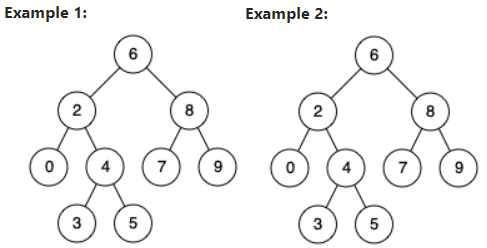
\includegraphics[width=0.80\textwidth]{lc-235-p-example.png} 
\caption{Example}
\label{Test}
\end{figure}

Example 1:

\begin{lstlisting}[language={python}]
Input: matrix = [["1","0","1","0","0"],["1","0","1","1","1"],["1","1","1","1","1"],["1","0","0","1","0"]]
Output: 6
Explanation: The maximal rectangle is shown in the above picture.
\end{lstlisting}

最大矩形如上圖所示。

Example 2:

\begin{lstlisting}[language={python}]
Input: matrix = []
Output: 0
\end{lstlisting}

Example 3:

\begin{lstlisting}[language={python}]
Input: matrix = [["0"]]
Output: 0
\end{lstlisting}

Example 4:

\begin{lstlisting}[language={python}]
Input: matrix = [["1"]]
Output: 1
\end{lstlisting}

Example 5:

\begin{lstlisting}[language={python}]
Input: matrix = [["0","0"]]
Output: 0
\end{lstlisting}

Constraints:

1. rows == matrix.length

2. cols == matrix[i].length

3. 1 <= row, cols <= 200

4. matrix[i][j] is '0' or '1'.

\subsection{LeetCode 235. 思路總結}

\subsection{LeetCode 235. Code 範例}

\begin{lstlisting}[language={python}]
class Solution(object):
    def lowestCommonAncestor(self, root, p, q):
        """
        :type root: TreeNode
        :type p: TreeNode
        :type q: TreeNode
        :rtype: TreeNode
        """
        if p.val<root.val and q.val<root.val:
            return self.lowestCommonAncestor(root.left,p,q)
        if p.val>root.val and q.val>root.val:
            return self.lowestCommonAncestor(root.right,p,q)
\end{lstlisting}

\subsection{LeetCode 235. 結果}

\begin{figure}[H]
\centering 
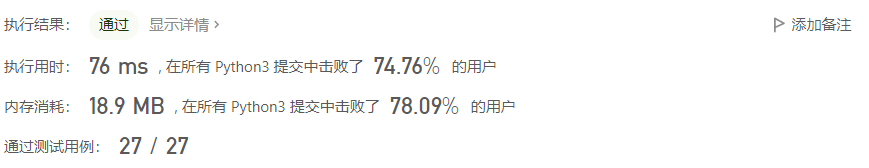
\includegraphics[width=0.80\textwidth]{lc-235-o.png} 
\caption{LeetCode 235 結果}
\label{Test}
\end{figure}


\newpage

\section{LeetCode 110. Balanced Binary Tree 平衡二叉樹}

\subsection{LeetCode 110. 題目}

Given an integer array nums, find a contiguous non-empty subarray within the array that has the largest product, and return the product.

The test cases are generated so that the answer will fit in a 32-bit integer.

A subarray is a contiguous subsequence of the array.

給你一個整數數組 nums,請你找出數組中乘積最大的非空連續子數組(該子數組中至少包含一個數字),並返回該子數組所對應的乘積。

測試用例的答案是一個 32-位 整數。

子數組 是數組的連續子序列。

\begin{figure}[H]
\centering 
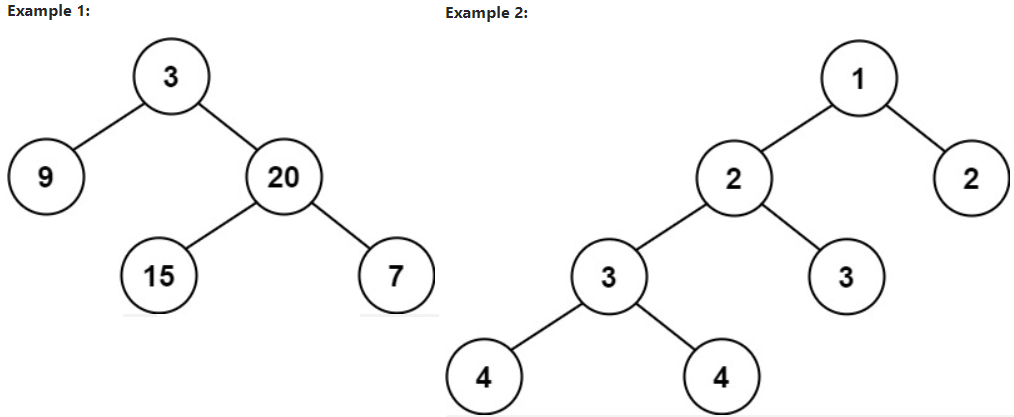
\includegraphics[width=0.80\textwidth]{lc-110-p-example.png} 
\caption{Example}
\label{Test}
\end{figure}


Example 1:

\begin{lstlisting}[language={python}]
Input: nums = [2,3,-2,4]
Output: 6
Explanation: [2,3] has the largest product 6.
子數組 [2,3] 有最大乘積 6。
\end{lstlisting}

Example 2:

\begin{lstlisting}[language={python}]
Input: nums = [-2,0,-1]
Output: 0
Explanation: The result cannot be 2, because [-2,-1] is not a subarray.
結果不能為 2, 因為 [-2,-1] 不是子數組。
\end{lstlisting}

Constraints:

1. $1 <= nums.length <= 2 * 10^{4}$

2. -10 <= nums[i] <= 10

3. The product of any prefix or suffix of nums is guaranteed to fit in a 32-bit integer.

nums 的任何前綴或後綴的乘積都 保證 是一個 32-位 整數

\subsection{LeetCode 110. 思路總結}

1. 給定一個整數數組 nums ,找出一個序列中乘積最大的連續子序列(該序列至少包含一個數)。

2. 給出一個數組,要求找出這個數組中連續元素乘積最大的值。

3. 這一題是 DP 的題,狀態轉移方程是:最大值是 Max(f(n)) = Max( Max(f(n-1)) * n, Min(f(n-1)) * n);最小值是 Min(f(n)) = Min( Max(f(n-1)) * n, Min(f(n-1)) * n)。只要動態維護這兩個值,如果最後一個數是負數,最大值就在負數 * 最小值中產生,如果最後一個數是正數,最大值就在正數 * 最大值中產生。

\subsection{LeetCode 110. Code 範例}

\begin{lstlisting}[language={python}]
class Solution:
    def maxProduct(self, A):
        B = A[::-1]
        for i in range(1, len(A)):
            A[i] *= A[i - 1] or 1
            B[i] *= B[i - 1] or 1
        return max(max(A),max(B)) 
\end{lstlisting}

\subsection{LeetCode 110. 結果}

\begin{figure}[H]
\centering 
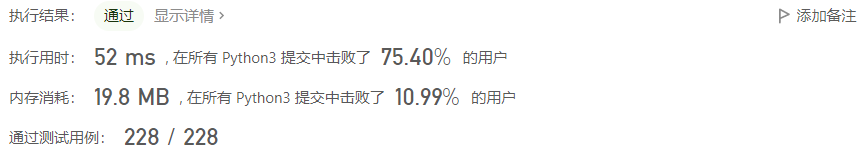
\includegraphics[width=0.80\textwidth]{lc-110-o.png} 
\caption{LeetCode 110 結果}
\label{Test}
\end{figure}


\newpage

\section{LeetCode 257. Binary Tree Paths 二叉樹的所有路徑}

\subsection{LeetCode 257. 題目}

Given an integer array nums, find a contiguous non-empty subarray within the array that has the largest product, and return the product.

The test cases are generated so that the answer will fit in a 32-bit integer.

A subarray is a contiguous subsequence of the array.

給你一個整數數組 nums,請你找出數組中乘積最大的非空連續子數組(該子數組中至少包含一個數字),並返回該子數組所對應的乘積。

測試用例的答案是一個 32-位 整數。

子數組 是數組的連續子序列。

\begin{figure}[H]
\centering 
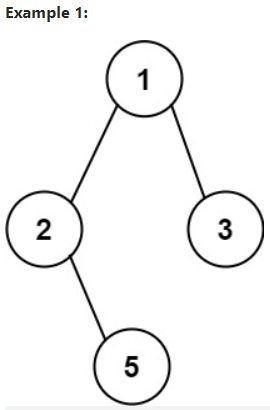
\includegraphics[width=0.30\textwidth]{lc-257-p-example.png} 
\caption{Example}
\label{Test}
\end{figure}


Example 1:

\begin{lstlisting}[language={python}]
Input: nums = [2,3,-2,4]
Output: 6
Explanation: [2,3] has the largest product 6.
子數組 [2,3] 有最大乘積 6。
\end{lstlisting}

Example 2:

\begin{lstlisting}[language={python}]
Input: nums = [-2,0,-1]
Output: 0
Explanation: The result cannot be 2, because [-2,-1] is not a subarray.
結果不能為 2, 因為 [-2,-1] 不是子數組。
\end{lstlisting}

Constraints:

1. $1 <= nums.length <= 2 * 10^{4}$

2. -10 <= nums[i] <= 10

3. The product of any prefix or suffix of nums is guaranteed to fit in a 32-bit integer.

nums 的任何前綴或後綴的乘積都 保證 是一個 32-位 整數

\subsection{LeetCode 257. 思路總結}

1. 給定一個整數數組 nums ,找出一個序列中乘積最大的連續子序列(該序列至少包含一個數)。

2. 給出一個數組,要求找出這個數組中連續元素乘積最大的值。

3. 這一題是 DP 的題,狀態轉移方程是:最大值是 Max(f(n)) = Max( Max(f(n-1)) * n, Min(f(n-1)) * n);最小值是 Min(f(n)) = Min( Max(f(n-1)) * n, Min(f(n-1)) * n)。只要動態維護這兩個值,如果最後一個數是負數,最大值就在負數 * 最小值中產生,如果最後一個數是正數,最大值就在正數 * 最大值中產生。

\subsection{LeetCode 257. Code 範例}

\begin{lstlisting}[language={python}]
class Solution:
    def maxProduct(self, A):
        B = A[::-1]
        for i in range(1, len(A)):
            A[i] *= A[i - 1] or 1
            B[i] *= B[i - 1] or 1
        return max(max(A),max(B)) 
\end{lstlisting}

\subsection{LeetCode 257. 結果}

\begin{figure}[H]
\centering 
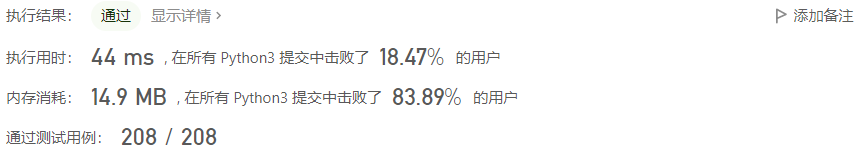
\includegraphics[width=0.80\textwidth]{lc-257-o.png} 
\caption{LeetCode 257 結果}
\label{Test}
\end{figure}



%\section{附錄}

% 數學意義說明

% $$\min \limits_{G}\max \limits_{D}{V_I(D,\ G)=V(D,G)-\lambda L_I(G,Q)}$$

%	\begin{lstlisting}[language={python}]

%	\end{lstlisting}

%\begin{enumerate}
%\item Y
%\item A
%\end{enumerate}

% \newpage

\clearpage

\end{document}